\documentclass{article}
\usepackage{amsmath}
\usepackage{graphicx}
\usepackage{booktabs}
\usepackage{siunitx}
\usepackage{pgfplotstable}

\sisetup{
	round-mode = places,
	round-precision = 2,
}

\title{My first document}
%\date{}
\author{Mo Khan}

\begin{document}
\pagenumbering{gobble}
\maketitle
\newpage
\tableofcontents
\newpage
\pagenumbering{arabic}

\section{Section}

Hello World!

\subsection{Subsection}

Structuring a document is easy!

\subsubsection{Subsubsection}

More text.

\paragraph{Paragraph}

Some more text.

\subparagraph{Subparagraph}

Even more text.

\newpage
\section{Another section}

\begin{equation*}
	f(x) = x^2
\end{equation*}

This is some example text\footnote{\label{myfootnote}Hello footnote}.

\begin{figure}[h!]
	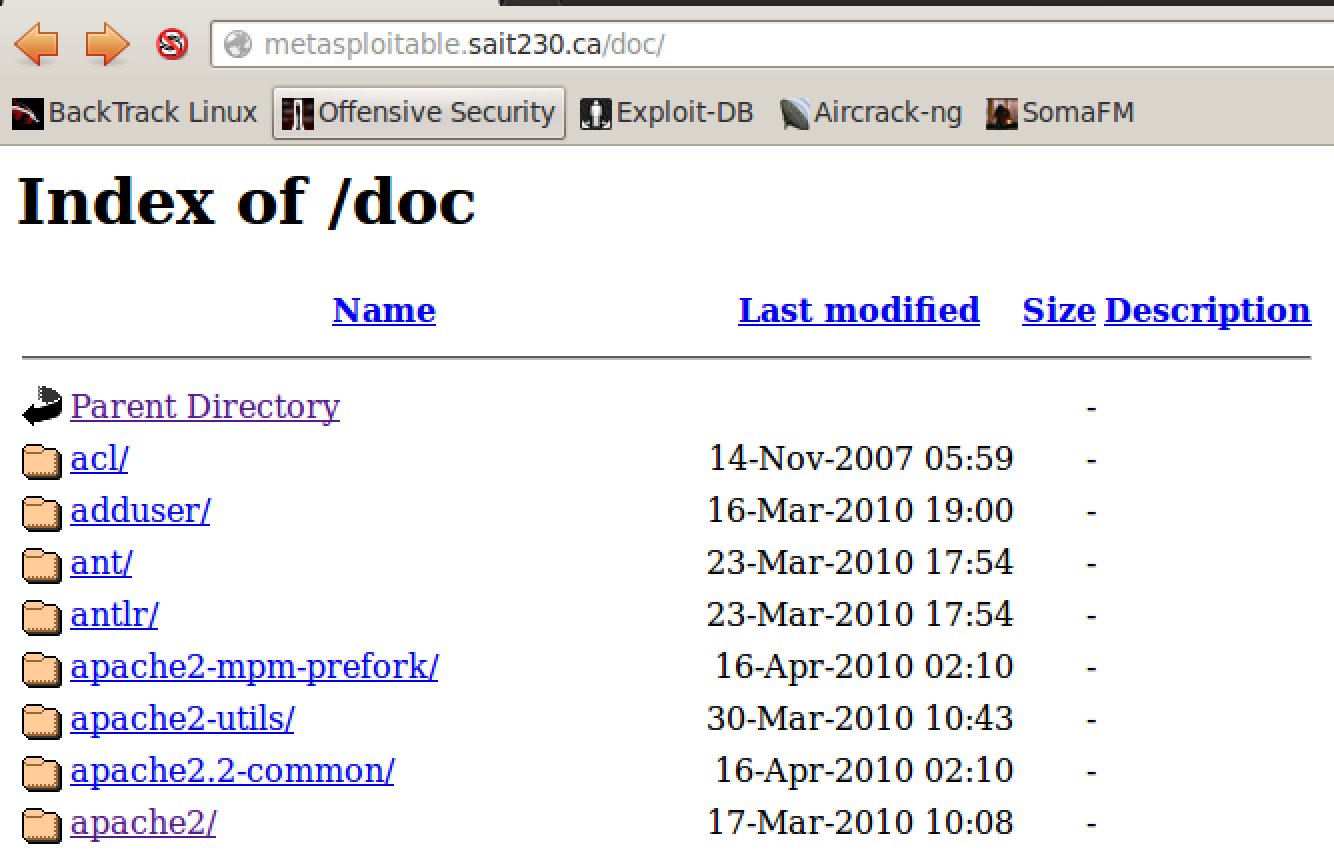
\includegraphics[width=\linewidth]{images/screenshot.png}
	\caption{A boat.}
	\label{fig:boat1}
\end{figure}

Figure \ref{fig:boat1} shows a boat.

\begin{table}[h!]
	\centering
	\caption{Caption for the table.}
	\label{tab:table1}
	\begin{tabular}{l|c||r}
		1 & 2 & 3\\
		\hline
		a & b & c\\
	\end{tabular}
\end{table}

I'm referring to footnote \ref{myfootnote}.

\begin{table}[h!]
	\centering
	\caption{Caption for the table.}
	\label{tab:table2}
	\begin{tabular}{ccc}
		\toprule
		Some & actual & content\\
		\midrule
		prettifies & the & content\\
		as & well & as\\
		using & the & booktabs package\\
		\bottomrule
	\end{tabular}
\end{table}

\newpage
\begin{table}
	\caption{Dummy table}
\end{table}

\begin{table}[h!]
	\begin{center}
		\caption{Autogenerated table from .csv file.}
		\label{table4}
		\pgfplotstabletypeset[
			multicolumn names, % allows to have multicolumn names
			col sep=comma, % the seperator in our .csv file
			display columns/0/.style={
				column name=$Value 1$, % name of first column
			column type={S},string type},  % use siunitx for formatting
			display columns/1/.style={
				column name=$Value 2$,
			column type={S},string type},
			every head row/.style={
				before row={\toprule}, % have a rule at top
				after row={
					\si{\ampere} & \si{\volt}\\ % the units seperated by &
				\midrule} % rule under units
			},
			every last row/.style={after row=\bottomrule}, % rule at bottom
		]{table.csv} % filename/path to file
	\end{center}
\end{table}

\newpage
\begin{appendix}
	\listoffigures
	\listoftables
\end{appendix}

\end{document}
